\section{Extensible Backend}
\subsection{Chat Bot}
\subsubsection{Process}
\begin{enumerate}
    \item{The user sends a query to the chat bot via the web interface.}
    \item{The chat bot backend extracts the keywords and intents from the query.}
    \item{It will then search the database to find candidate responses.}
    \item{A score is calculated for each candidate based on its theta value and salience.}
    \item{The candidate with the highest score is considered the best answer.}
    \item{When deciding on a response, the chat bot also considers whether or not the user's query is a question.}
    \item{The final chosen answer is returned to the user via the web interface.}
\end{enumerate}

\subsubsection{Example Usage}
The user accesses the chat interface and sends a greeting message. This is parsed and detected as a "Default Welcome Intent", and the bot responds accordingly.

\begin{center}
    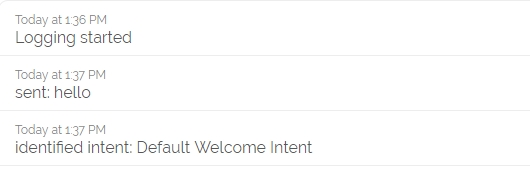
\includegraphics[width=7cm]{log1.png}
\end{center}

The user then asks "What is fork?" This query is also processed and the intent is identified as corresponding to the course content. The chat bot queries the database and chooses from the answers with the highest score. The answer with the highest score is displayed at the top in the debug log shown below.

\begin{center}
    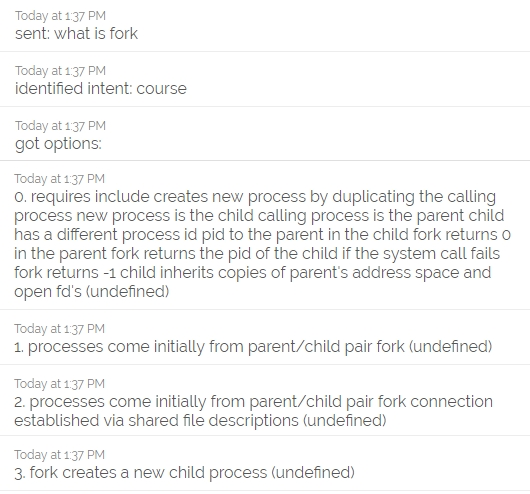
\includegraphics[width=7cm]{log2.png}
\end{center}

\subsubsection{Technical Details}
The salience value for keywords is calculated using the tf-idf algorithm. 

\subsection{Internal APIs}
\subsubsection{Process}
\begin{enumerate}
    \item{}
\end{enumerate}

\subsubsection{Usage}

\subsubsection{Technical Details}
% refer to appendix
We have constructed a backend in \code{Javascript} using \code{Node.js}. This runs on an \code{EC2} instance on Amazon Web Services (AWS). 
\newpage
